
与内存数据相比,CPU中的寄存器可以更快地对数据进行操作。处理器和内存的速度至少有一个数量级的差异,在没有通过直接测量对性能进行验证之前,不要对性能做出任何猜测或假设。不过这不意味着关于系统架构的先验知识和基于这些知识的假设都没用,假设可以用来指导实验和设计正确的测试方法。我们将在本章中了解到,偶然尝到的甜头不会走太远,甚至会误入歧途。测试本身没问题,但通常很难确定测量的是什么,以及可以从结果中得出什么结论。

测量内存访问速度相当简单,需要一些可以读取内存和确定读取时间的方法,像这样:

\begin{lstlisting}[style=styleCXX]
volatile int* p = new int;
*p = 42;
for (auto _ : state) {
	benchmark::DoNotOptimize(*p);
}
delete p;
\end{lstlisting}

这个基准测试会运行和测试……一些东西。可以将一次迭代的时间报告为0纳秒。这可能是不必要的编译器优化结果。如果编译器发现整个程序没有可观察行为,那么确实可以将其优化为零。但是,针对这样的事件采取了措施。读取的内存是\texttt{volatile},访问\texttt{volatile}内存会认为是一种可观察行为,不能优化掉。相反,0纳秒的结果在一定程度上是基准测试本身的缺陷,表明单次读取的速度要快于1纳秒。这里测试到的内存速度与期望大相径庭,我们不能从一个什么都没有的报告中得到任何东西,包括自己犯的错误。在修正基准测试方面,我们要做的就是在基准测试迭代中进行多次读取,如下所示:

\begin{lstlisting}[style=styleCXX]
volatile int* p = new int;
*p = 42;
for (auto _ : state) {
	benchmark::DoNotOptimize(*p);
	… repeat 32 times …
	benchmark::DoNotOptimize(*p);
}
state.SetItemsProcessed(32*state.iterations());
delete p;
\end{lstlisting}

每次迭代执行32次读取,可以从报告的迭代时间中计算出单个读取的时间。让谷歌基准库为我们进行计算,并报告每秒读取的次数。这可以通过在基准测试结束时,设置处理数量来实现。

基准测试在中等级别的CPU上,大约需要5纳秒的迭代时间,从而确认单次读取时间是总时间的1/32,远低于1纳秒(因此对每次迭代报告为0的猜测得到了验证)。另一方面,这个值与我们对慢速内存的期望并不匹配,所以我们之前关于性能瓶颈的假设可能不正确,当然还可以测试内存速度之外的指标。

\subsubsubsection{4.3.1\hspace{0.2cm}内存架构}

为了理解如何正确地测试内存性能,必须更多地了解现代处理器的内存架构,内存系统最重要的特性是层级结构。CPU不直接访问主存,而是通过缓存的层级结构进行:

%\hspace*{\fill} \\ %插入空行
\begin{center}
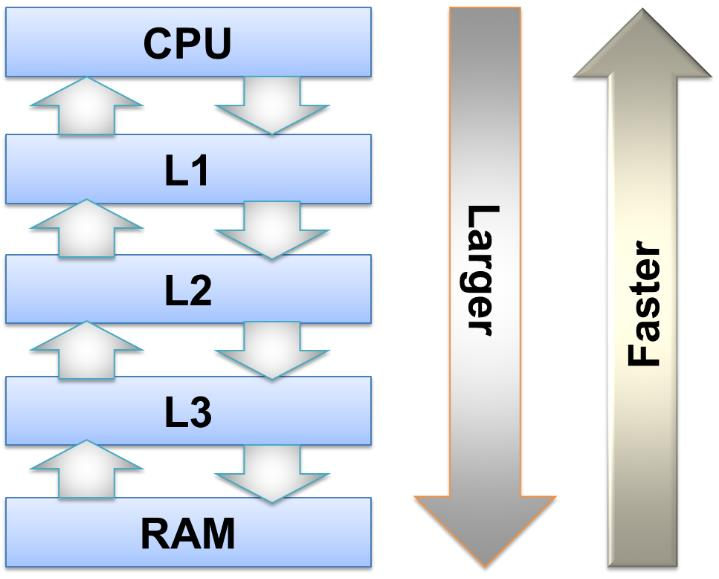
\includegraphics[width=0.5\textwidth]{content/1/chapter4/images/2.jpg}\\
图4.2 - 内存层级结构图
\end{center}

图4.2中的\textbf{RAM}是主存储器,即主板上的DRAM。系统说明书上说,这台机器有这么多G的内存,这就是DRAM的容量。可以看到,CPU并不直接访问主内存,而是通过几个层级结构的缓存访问主内存。这些缓存也是内存电路,但它们位于CPU芯片内部,使用不同的技术来存储数据,都是不同速度的SRAM。DRAM和SRAM的关键区别在于SRAM的访问速度要快得多,但比DRAM的功耗要大得多。随着我们在内存层级结构中越靠近CPU,内存访问的速度就越快。level-1(\textbf{L1})缓存的访问时间与CPU寄存器的访问时间几乎相同,但它功耗很大,以至于只能拥有几千字节的内存空间,通常每个CPU核心有32KB的L1缓存。下一层,\textbf{L2}缓存更大但更慢,第三层(\textbf{L3})缓存更大但也更慢(通常在CPU的多核之间共享),层次结构的最后一层就是主存。

CPU第一次从主内存中读取数据值,该值通过所有缓存级别传播,其副本保留在缓存中。CPU再次读取相同的值,不需要等待从主内存获取值,因为相同值的副本已经存储在L1缓存中。

读取的数据需要适合L1缓存的长度,所有数据在第一次访问时就会加载到缓存中,之后CPU只需要访问L1缓存即可。如果访问不在缓存中的值,并且缓存已满,那么必须从缓存中清除一些内容,为新值腾出空间。这个过程完全由硬件控制,它有一些方法,根据我们最近访问的值(根据第一次近似,长时间没有使用的数据可能很快就不再需要了),来确定我们最不可能再次需要哪个值。下一级缓存更大,但使用方式相同:只要数据在缓存中,就在那里访问它(离CPU越近越好)。否则,需要从下一级缓存取值,对于L3缓存来说,就是从主存取值,如果缓存已满,一些其他的数据块必须从缓存中去除(也就是被缓存遗忘,不过原始数据仍在主存中)。

由于反复读取相同的值成千上万次,初始读取的时间基本上可以忽略,测试所得的平均读取时间是L1缓存的读取时间。L1缓存的速度确实非常快,所以如果测试数据是32KB,就不需要担心内存的读取的性能差。不过,还是需要了解如何正确地测量内存性能,这样才能得出相应的结论。

\subsubsubsection{4.3.2\hspace{0.2cm}测试内存和缓存的速度}

已经理解了内存速度比一次读取的时间要复杂得多,现在可以设计一个更合适的基准测试。可以预期缓存大小会对结果有影响,因此必须访问不同大小的数据,从几千字节(适合32KB的L1缓存)到几十兆字节或更多(L3缓存大小不同,但通常在8MB到12MB之间)。由于对于大数据量测试,内存系统将从缓存中清除旧数据,所以可以预期性能取决于预测的情况,或者说取决于访问模式。所谓的访问,例如复制一个内存范围,可能会以非常不同方式结束,而不是以随机的顺序访问相同的范围。最后,结果可能取决于内存访问的粒度,访问64位的值比访问单个字符,哪个快?

连续读取大数组的基准测试:

\hspace*{\fill} \\ %插入空行
\noindent
\textbf{01c\_cache\_sequential\_read.C}
\begin{lstlisting}[style=styleCXX]
template <class Word>
void BM_read_seq(benchmark::State& state) {
	const size_t size = state.range(0);
	void* memory = ::malloc(size);
	void* const end = static_cast<char*>(memory) + size;
	volatile Word* const p0 = static_cast<Word*>(memory);
	Word* const p1 = static_cast<Word*>(end);
	for (auto _ : state) {
		for (volatile Word* p = p0; p != p1; ) {
			REPEAT(benchmark::DoNotOptimize(*p++);)
		}
		benchmark::ClobberMemory();
	}
	::free(memory);
	state.SetBytesProcessed(size*state.iterations());
	state.SetItemsProcessed((p1 - p0)*state.iterations());
}
\end{lstlisting}

编写的基准测试与之前非常类似,只是在主循环中做了一行修改:

\hspace*{\fill} \\ %插入空行
\noindent
\textbf{01d\_cache\_sequential\_write.C}
\begin{lstlisting}[style=styleCXX]
Word fill = {}; // Default-constructed
for (auto _ : state) {
	for (volatile Word* p = p0; p != p1; ) {
		REPEAT(benchmark::DoNotOptimize(*p++ = fill);)
	}
	benchmark::ClobberMemory();
}
\end{lstlisting}

写入数组的值并不重要。如果认为0有点特殊,那么可以用其他值初始化\texttt{fill}。

使用\texttt{REPEAT}宏来避免多次手动复制代码。我们仍然希望每次迭代执行几次内存读取。当开始报告每秒读取的数量时,避免每次迭代0纳秒的报告就不重要了,但是对于这样成本非常低的迭代来说,循环本身的开销并不小,所以最好手动展开这个循环。\texttt{REPEAT}宏将循环展开32次:

\begin{lstlisting}[style=styleCXX]
#define REPEAT2(x) x x
#define REPEAT4(x) REPEAT2(x) REPEAT2(x)
#define REPEAT8(x) REPEAT4(x) REPEAT4(x)
#define REPEAT16(x) REPEAT8(x) REPEAT8(x)
#define REPEAT32(x) REPEAT16(x) REPEAT16(x)
#define REPEAT(x) REPEAT32(x)
\end{lstlisting}

当然,必须确保请求的内存大小足够容纳32个\texttt{Word}类型的值,并且数组的总大小能被32整除,这对基准测试代码来说都不是什么限制。

说到\texttt{Word}类型,这是第一次使用\texttt{TEMPLATE}基准测试。它用于在不复制代码的情况下为几种类型生成基准测试:

\begin{lstlisting}[style=styleCXX]
#define ARGS ->RangeMultiplier(2)->Range(1<<10, 1<<30)
BENCHMARK_TEMPLATE1(BM_read_seq, unsigned int) ARGS;
BENCHMARK_TEMPLATE1(BM_read_seq, unsigned long) ARGS;
\end{lstlisting}

如果CPU支持,可以在更大的块中读写数据,例如:在x86 CPU上使用SSE和AVX指令一次移动16或32个字节。在GCC或Clang中,对于这些较大的类型,有一些头文件:

\begin{lstlisting}[style=styleCXX]
#include <emmintrin.h>
#include <immintrin.h>
…
BENCHMARK_TEMPLATE1(BM_read_seq, __m128i) ARGS;
BENCHMARK_TEMPLATE1(BM_read_seq, __m256i) ARGS;
\end{lstlisting}

\texttt{\_\_m128i}和\texttt{\_\_m256i}类型没内置在语言中(至少不是C/C++),但C++可以很容易地声明新类型。这些是值类型类(表示单个值的类),有一组定义好的算术操作(加法和乘法),编译器使用适当的SIMD指令来实现这些操作。

前面的基准测试依次访问内存范围,从开始到结束。内存的大小随基准参数的指定而变化(在本例中,从1KB到1GB,每次增加一倍)。当复制一定范围的内存时,基准测试会从头再做一次,直到积累足够的量。

当以随机顺序测量访问内存速度,必须小心。天真的对代码进行基准测试看起来可能会像这样:

\begin{lstlisting}[style=styleCXX]
benchmark::DoNotOptimize(p[rand() % size]);
\end{lstlisting}

但此基准测试了调用\texttt{rand()}函数所需的时间,计算开销比读取单个整数要大得多,因此可能永远不会注意到后者的开销。取模运算符\texttt{\%}比单个读或写开销大得多。获得精确结果的唯一方法是预先计算随机索引,并将它们存储在另一个数组中。当然,现在正在同时读取索引值和索引数据,所以测量的开销是两次读取(或一次读取和一次写入)。

随机写入内存的代码如下所示:

\hspace*{\fill} \\ %插入空行
\noindent
\textbf{01b\_cache\_random\_write.C}
\begin{lstlisting}[style=styleCXX]
const size_t N = size/sizeof(Word);
std::vector<int> v_index(N);
for (size_t i = 0; i < N; ++i) v_index[i] = i;
std::random_shuffle(v_index.begin(), v_index.end());
int* const index = v_index.data();
int* const i1 = index + N;
Word fill; memset(&fill, 0x0f, sizeof(fill));
for (auto _ : state) {
	for (const int* ind = index; ind < i1; ) {
		REPEAT(*(p0 + *ind++) = fill;)
	}
	benchmark::ClobberMemory();
}
\end{lstlisting}

使用STL算法\texttt{random\_shuffle}来产生随机的索引顺序(可以用随机数代替,这并不完全相同,因为一些指数可能出现过不止一次,而另一些则从未出现过,但这不会对结果产生太大影响)。处理的值实际上不重要,编写任何数字都需要相同的时间,但是编译器有时可以进行优化,如果它能够发现代码出现了大量的零,那么最好避免这种情况。另外,较长的AVX类型不能用整数初始化,因此可以使用\texttt{memset()}写入值。

当然,读取的基准测试代码非常相似,只是内部循环进行了修改:

\begin{lstlisting}[style=styleCXX]
REPEAT(benchmark::DoNotOptimize(*(p0 + *ind++));)
\end{lstlisting}

基准测试代码主要用于测量内存访问的开销,而对索引的运算不可避免,但是加法最多只需要一个时钟周期(CPU可以同时做几个),所以数学运算不会成为瓶颈(而且,访问数组内存的程序都必须做相同的计算,因此这就是实际中的访问速度)。来看看结果吧!




























